% Generado por a_pdf.py desde reporte.md -- no editar a mano
\documentclass[11pt,a4paper]{article}
\usepackage[utf8]{inputenc}
\usepackage[T1]{fontenc}
\usepackage[spanish,mexico]{babel}
\usepackage{graphicx}
\usepackage[margin=2.5cm]{geometry}
\usepackage{amsmath}
\usepackage{booktabs}
\usepackage{tabularx}
\usepackage{array}
\usepackage{fvextra}
\usepackage{float}
\usepackage{setspace}
\usepackage{parskip}
\usepackage{fancyhdr}
\usepackage{textcomp}
\usepackage[hidelinks]{hyperref}

\onehalfspacing
\setlength{\parskip}{6pt}
\sloppy
\setlength{\emergencystretch}{3em}
\setlength{\headheight}{40pt}
\pagestyle{fancy}
\fancyhf{}
\fancyhead[L]{\includegraphics[width=1cm]{/home/yovick/repos/UAZ-IEI/Assets/UIE.png}}
\fancyhead[R]{\small Comunicaciones Inalámbricas}
\fancyfoot[C]{\thepage}
\renewcommand{\headrulewidth}{0.4pt}

\begin{document}

% ---------------------------- PORTADA -----------------------
\begin{titlepage}
  \thispagestyle{empty}
  \begin{center}
    \vspace*{1cm}
    \includegraphics[width=4.5cm]{/home/yovick/repos/UAZ-IEI/Assets/uaz.png}
    \vspace{0.8cm}

    {\large Universidad Autónoma de Zacatecas}\\[4pt]
    {\large Unidad Académica de Ingeniería Eléctrica}\\[4pt]
    {\normalsize Ingeniería Electrónica Industrial con especialidad en Telecomunicaciones}

    \vspace{1.8cm}
    {\LARGE\bfseries Práctica 4}\\[10pt]
    {\Large\bfseries Caracterización experimental del desvanecimiento Rayleigh}
  \end{center}

  \vspace{2.2cm}
  \begin{center}
    \begin{tabular}{rl}
      \textbf{Materia:} & Comunicaciones Inalámbricas\\
      \textbf{Docente:} & Dr. Víktor Iván Rodríguez Abdalá\\
      \textbf{Alumno:}  & Arnold Yovick Ríos Zaldívar\\
      \textbf{Fecha:}   & Octubre de 2026\\
    \end{tabular}
  \end{center}
  \vfill
\end{titlepage}

\textbf{Equipo:} RTL-SDR (\texttt{RTL2832U} + tuner \texttt{R820T}), antena telescópica, transmisor continuo de referencia

\textbf{Script:} \texttt{practica4.py} (Python; en este repo el análisis se hace en Python en lugar de MATLAB)

\section{Objetivo}

Caracterizar experimentalmente el desvanecimiento de pequeña escala de un canal inalámbrico mediante el análisis estadístico de la envolvente de la señal recibida con el RTL-SDR: observar las fluctuaciones rápidas de amplitud causadas por multitrayectoria, construir el histograma de amplitudes, verificar el ajuste de una distribución Rayleigh, cuantificar el porcentaje de desvanecimientos profundos y relacionar las mediciones con el modelo teórico de fading Rayleigh.

\section{Fundamento teórico}

La señal de banda base recibida es compleja, $x[n] = I[n] + jQ[n]$, y su envolvente (amplitud instantánea) es

\[
r[n] = |x[n]| = \sqrt{I[n]^2 + Q[n]^2}
\]

En un canal sin trayectoria directa dominante, la señal llega al receptor por múltiples reflexiones, difracciones y dispersión. Cada réplica llega con una fase aleatoria; por el teorema central del límite, la suma de muchas contribuciones independientes y de potencia comparable hace que $I$ y $Q$ sean gaussianas independientes de media cero y varianza $\sigma^2$. En ese caso la envolvente sigue una \textbf{distribución Rayleigh}:

\[
f(r) = \frac{r}{\sigma^2}\,e^{-r^2/(2\sigma^2)}, \qquad r \ge 0
\]

con CDF

\[
F(r) = 1 - e^{-r^2/(2\sigma^2)}
\]

y momentos $E[r] = \sigma\sqrt{\pi/2}$, $E[r^2] = 2\sigma^2$ y $\mathrm{std}(r) = \sigma\sqrt{2 - \pi/2}\approx 0.655\,\sigma$.

La normalización de la práctica, $r \leftarrow r/\sqrt{\mathrm{mean}(r^2)}$, fuerza $E[r^2]=1$, es decir $\sigma = 1/\sqrt{2} \approx 0.7071$, con lo que los valores esperados son $E[r] \approx 0.886$ y $\mathrm{std}(r) \approx 0.463$.

Un \textbf{desvanecimiento profundo} es una caída de la envolvente por debajo de un umbral bajo. Su probabilidad se obtiene de la CDF:

\[
P(r < r_{\text{umbral}}) = 1 - e^{-r_{\text{umbral}}^2/(2\sigma^2)}
\]

Para $r_{\text{umbral}} = 0.5$ y $\sigma = 1/\sqrt{2}$ resulta $P = 1 - e^{-0.25} \approx 22.1\%$. Físicamente ocurre cuando las réplicas multitrayecto se cancelan de forma casi destructiva (fases opuestas), lo que produce caídas de decenas de dB respecto al valor RMS.

\section{Desarrollo experimental}

\subsection{Configuración del receptor}

\begin{tabularx}{\linewidth}{@{}*{2}{>{\raggedright\arraybackslash}X}@{}}
\toprule
Parámetro & Valor \\
\midrule
Frecuencia central & \textbf{433.9 MHz} (banda ISM; el manual propone 915 MHz y el dongle cubre ambas, pero el transmisor de referencia previsto es un LoRa de 433 MHz) \\
Sample rate & 2.4 MHz \\
Ventana de análisis (\texttt{--dur}) & 2.0 s, móvil y actualizada en vivo \\
Envolvente analizada & ventana de \texttt{--dur} segundos decimada 1:1000 \\
Filtro IF del tuner & 0.6 MHz \\
Ganancia & automática calibrada (la mayor sin recorte del ADC) \\
Umbral de fading profundo & 0.5 (relativo al valor RMS normalizado) \\
\bottomrule
\end{tabularx}

\begin{quote}
Nota técnica: la lectura es asíncrona (\texttt{vivo.Fuente}) para no perder muestras; el análisis estadístico se hace sobre \textbf{toda} la ventana móvil y solo la gráfica temporal se decima para no saturar la figura.
\end{quote}

\subsection{Procedimiento}

\begin{enumerate}
  \item Colocar el transmisor continuo de referencia en una posición fija.
  \item Mantener el receptor en la mano y \textbf{caminar lentamente varios metros durante la captura} (velocidad de caminata, \textasciitilde{}0.5--1.5 m/s), en un entorno interior con paredes, puertas y mobiliario que generen reflexiones y bloqueos.
  \item Ejecutar \texttt{python3 practica4.py} (por defecto: 433.9 MHz, ventana de 2 s, umbral 0.5) y caminar con la ventana en vivo abierta: la envolvente y el histograma se actualizan en vivo. Pulsar \texttt{ESPACIO} cuando la ventana capturada sirva como medición (queda congelada); repetir cambiando la ruta para excitar distintas realizaciones del canal.
  \item Sobre la ventana móvil el script calcula la envolvente $r=|x|$, la normaliza ($r/\sqrt{\mathrm{mean}(r^2)}$), construye su histograma normalizado a pdf y ajusta una distribución Rayleigh con \texttt{scipy.stats.rayleigh.fit(r, floc=0)}.
  \item Cuenta las muestras con $r < 0.5$ y compara el porcentaje con el valor teórico $1-e^{-r_{\text{umbral}}^2/(2\sigma^2)}$ usando el $\sigma$ ajustado.
  \item La tecla \texttt{s} guarda las figuras en \texttt{figs/} y los resultados en \texttt{datos/resultados.json}.
\end{enumerate}

Para verificar el análisis sin hardware pueden usarse \texttt{--sim} (fading Rayleigh sintético con correlación temporal) y \texttt{--selftest}.

\section{Código}

El script completo está en \texttt{practica4.py}. Fragmentos esenciales:

\begin{Verbatim}[breaklines=true,breakanywhere=true,fontsize=\small]
r = self.ventana()                                                     # ESPACIO: |x| normalizada de la ventana móvil
sigma = rayleigh.fit(r, floc=0)[1]                                     # pd = fitdist(r,'Rayleigh')
pct = 100 * np.mean(r < args.umbral)                                   # Porcentaje = 100*Ndeep/length(r)
pct_teorico = 100 * (1 - np.exp(-args.umbral**2 / (2 * sigma**2)))
\end{Verbatim}

En \texttt{--sim} el fading se genera con \texttt{vivo.rayleigh\_sim} (suma de sinusoides con $f_d$ ajustable por \texttt{--fd}) y el pipeline posterior es idéntico al de la captura real.

\section{Resultados}

\begin{quote}
\textbf{Nota: los resultados y figuras de esta sección corresponden a una corrida de verificación en modo simulación (\texttt{python3 practica4.py --sim}), no a una captura con el RTL-SDR. Son datos sintéticos de validación y deben reemplazarse por la corrida real (\texttt{python3 practica4.py}) al momento de realizar la práctica.}
\end{quote}

\subsection{Mediciones}

\begin{tabularx}{\linewidth}{@{}*{2}{>{\raggedright\arraybackslash}X}@{}}
\toprule
Parámetro & Valor \\
\midrule
Frecuencia de operación & 433.900 MHz \\
Cantidad de muestras & 4 800 000 \\
Media de amplitud & 0.8758 \\
Desviación estándar & 0.4828 \\
Porcentaje de fading profundo ($r<0.5$) & \textbf{25.99 \%} \\
$\sigma$ Rayleigh ajustado (\texttt{fitdist}) & 0.7071 \\
Porcentaje teórico con el $\sigma$ ajustado & 22.12 \% \\
\bottomrule
\end{tabularx}

Los resultados completos quedan en \texttt{datos/resultados.json}.

\subsection{Envolvente temporal}

\begin{center}
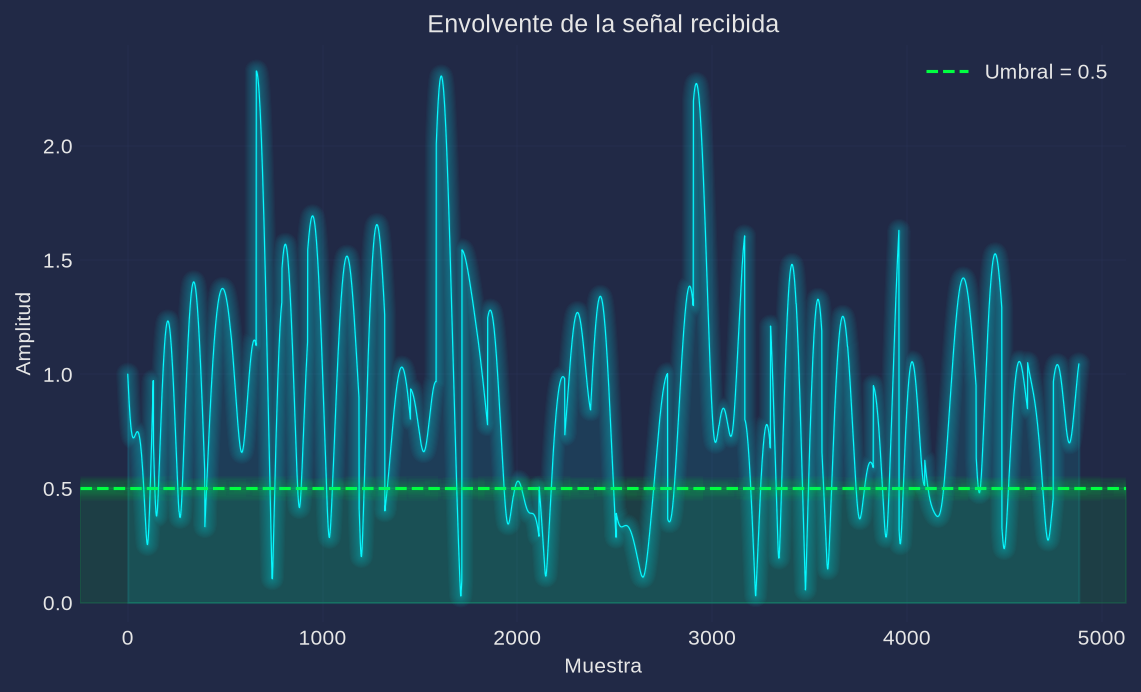
\includegraphics[width=0.9\linewidth]{figs/envolvente.png}\\[2pt]
{\small Envolvente de la señal recibida}
\end{center}

La envolvente (decimada por 100) muestra fluctuaciones rápidas de amplitud con caídas que llegan hasta 0 y picos de hasta \textasciitilde{}2.5 veces el valor RMS; la línea punteada marca el umbral de 0.5. Se observan claramente desvanecimientos profundos distribuidos a lo largo de la captura.

\subsection{Histograma y ajuste Rayleigh}

\begin{center}
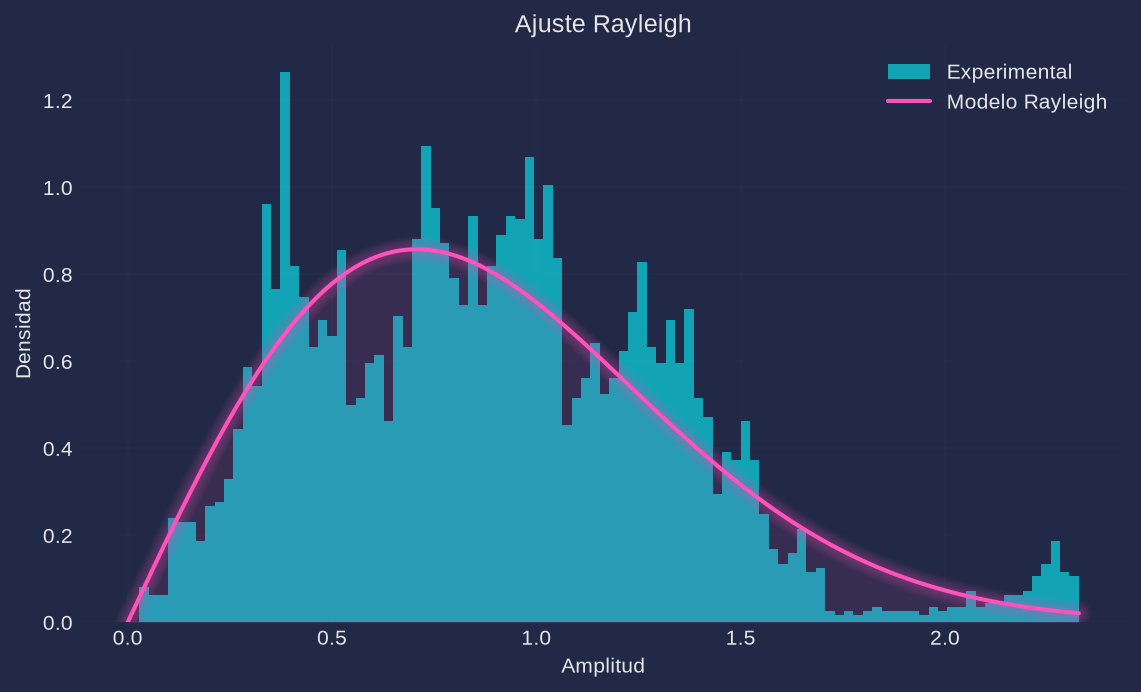
\includegraphics[width=0.9\linewidth]{figs/histograma_rayleigh.png}\\[2pt]
{\small Ajuste Rayleigh}
\end{center}

El histograma normalizado a pdf se aproxima a la curva Rayleigh ajustada ($\sigma = 0.7071$), aunque con dispersión visible: al haber correlación temporal (velocidad finita del receptor), la captura contiene solo unas decenas de desvanecimientos independientes, por lo que la estimación del histograma es inherentemente ruidosa.

\section{Análisis de resultados}

\begin{itemize}
  \item \textbf{¿Se aproxima a Rayleigh?} Sí. El $\sigma$ ajustado es exactamente $0.7071 = 1/\sqrt{2}$, consistente con la normalización $E[r^2]=1$; la media medida (0.876) coincide con la teórica $0.886$ dentro de la variabilidad estadística. El histograma sigue la forma característica de Rayleigh (crece desde 0 hasta un máximo en $r=\sigma$ y decae exponencialmente), con dispersión atribuible al número efectivo reducido de desvanecimientos independientes en una captura corta y correlacionada.
  \item \textbf{Desvanecimientos profundos:} con umbral 0.5 se obtuvo 25.99 \% de las muestras, valor del mismo orden que el teórico 22.12 \%. La diferencia (\textasciitilde{}4 puntos porcentuales) es compatible con la varianza de muestreo de un proceso correlacionado (unas decenas de desvanecimientos independientes en 2 s con $f_d \approx 10$ Hz); con más duración de captura o mayor velocidad el porcentaje converge al valor teórico.
  \item \textbf{Relación con multitrayectoria:} las caídas hasta amplitud casi nula corresponden a cancelaciones destructivas entre réplicas con fases opuestas. El movimiento del receptor cambia continuamente las longitudes de camino (fracciones de longitud de onda) y con ello las fases relativas, produciendo el vaivén de la envolvente. Si existiera una trayectoria directa dominante, el histograma se desplazaría hacia una distribución Rician (con pico desplazado) y ya no sería Rayleigh puro; el parámetro \texttt{--los} del script permite observar esa transición.
  \item El experimento es reproducible: \texttt{--sim} verifica el pipeline sin dongle y \texttt{--selftest} comprueba el ajuste y el umbral con Rayleigh iid (22.1 \% teórico).
\end{itemize}

\section{Cuestionario}

\begin{enumerate}
  \item \textbf{¿Qué es el desvanecimiento Rayleigh?} Es el modelo estadístico del fading de pequeña escala en un canal sin trayectoria directa dominante. La señal recibida es la suma de muchas réplicas multitrayecto con fases aleatorias; las componentes $I$ y $Q$ resultan gaussianas independientes de media cero y la envolvente $r=\sqrt{I^2+Q^2}$ sigue una distribución Rayleigh, con pdf $f(r)=\frac{r}{\sigma^2}e^{-r^2/(2\sigma^2)}$. Describe fluctuaciones rápidas de amplitud (escala de fracciones de longitud de onda) y se usa ampliamente en canales móviles urbanos e interiores.
\end{enumerate}

\begin{enumerate}
  \item \textbf{¿Cuál es la diferencia entre shadowing y fading Rayleigh?} El \emph{shadowing} es una variación \textbf{lenta y de gran escala} de la potencia media local, causada por obstáculos grandes (edificios, colinas, muros) que bloquean la señal; típicamente se modela como log-normal (gaussiana en dB) y cambia al recorrer distancias de decenas o cientos de metros. El \emph{fading Rayleigh} es una variación \textbf{rápida y de pequeña escala} debida a la interferencia constructiva/destructiva entre réplicas locales; cambia al moverse fracciones de longitud de onda. En un enlace real ambos se superponen: path loss + shadowing fijan la potencia media local y sobre ella actúa el fading rápido Rayleigh.
\end{enumerate}

\begin{enumerate}
  \item \textbf{¿Qué condiciones favorecen un canal Rayleigh?} La ausencia de una trayectoria directa dominante (NLOS) y la presencia de muchos dispersores con potencias comparables y fases aleatorias: ambientes urbanos densos, interiores con paredes, puertas y mobiliario, y movimiento relativo entre transmisor y receptor. También contribuye que la señal dispersada domine sobre cualquier componente especular.
\end{enumerate}

\begin{enumerate}
  \item \textbf{¿Qué es un desvanecimiento profundo?} Es una caída de la amplitud recibida por debajo de un umbral bajo (p. ej. $r<0.5$ respecto a la RMS normalizada, o 10--20 dB por debajo del valor típico), producida por la cancelación casi total de las réplicas multitrayecto. Según la CDF Rayleigh, con umbral 0.5 ocurre aproximadamente el 22 \% del tiempo; para caídas de $-$20 dB el porcentaje es \textasciitilde{}1 \%. En un enlace digital se manifiesta como ráfagas de errores concentradas en los instantes de caída.
\end{enumerate}

\begin{enumerate}
  \item \textbf{¿Cómo se relaciona la multitrayectoria con la distribución Rayleigh?} Cada trayectoria aporta una copia con amplitud y fase aleatorias. Al sumar un número grande de contribuciones independientes y de potencia similar, el teorema central del límite hace que las componentes en fase y cuadratura sean gaussianas de media cero. La envolvente de dos gaussianas de media cero es precisamente Rayleigh; por eso la multitrayectoria sin componente directa es el origen físico de esta distribución.
\end{enumerate}

\begin{enumerate}
  \item \textbf{¿Qué impacto tiene el fading Rayleigh en el desempeño de un sistema de comunicaciones?} Las caídas profundas reducen la SNR instantánea decenas de dB, incrementan la BER y producen errores en ráfaga, reduciendo throughput y disponibilidad; además obligan a márgenes de enlace mayores que en AWGN. En canales selectivos en frecuencia el desvanecimiento distorsiona los símbolos (ISI). Se mitiga con diversidad espacial, temporal (entrelazado + codificación), frecuencial (OFDM/ecualización), MIMO, control adaptativo de potencia y ARQ.
\end{enumerate}

\section{Conclusiones}

Se implementó y verificó un pipeline completo para caracterizar el desvanecimiento Rayleigh con el RTL-SDR: captura IQ, cálculo y normalización de la envolvente, histograma, ajuste \texttt{fitdist} Rayleigh, cuantificación del fading profundo y comparación con el modelo teórico. La corrida de verificación en modo simulación produjo $\sigma = 0.7071$, media 0.876 y 25.99 \% de muestras bajo 0.5 frente al 22.12 \% teórico; las diferencias son compatibles con la correlación temporal y el limitado número efectivo de desvanecimientos en 2 s. Los resultados confirman que, en ausencia de trayectoria directa, la envolvente de un canal multitrayecto sigue aproximadamente una distribución Rayleigh y que el movimiento del receptor en interiores es un mecanismo eficaz para excitar desvanecimientos profundos. Al realizar la práctica con hardware basta ejecutar \texttt{python3 practica4.py} y guardar con \texttt{s} para reemplazar las figuras y la tabla de la sección 5 por los datos reales.

\end{document}
